\documentclass{article}
\usepackage{graphicx}
\title{MCM Trading problem}
\author{Ahad Jiva}
\graphicspath{../latex/}
\begin{document}
\maketitle

\section*{Problem Summary}
With the data given, the goal is to develop a mathematical model that makes optimal daily trades using only previous price data. 
\$1000 is given at the start, and the model must make as much profit as possible.

\section*{Solution}
This solution uses mean reversion, the idea that asset prices in the long run will revert to their averages. Using the five years of price data given, a moving average is tracked as time passes and the model will either buy if the price is below the average or sell if above the average. The size of the moving average window is a parameter that affects model performance.

\section*{Equations}
The n-day moving average is defined as
\begin{equation}
    \frac{p_1 + p_2 + ... + p_n}{n}
\end{equation}
where each $p_k$ is the price of the asset on a specific day. The model also has the ability to use exponential moving averages, which assign weights to previous
prices depending on how recent they are. Exponential moving averages are calculated recursively and defined as
\begin{equation}
    e_k = \left(p_k \cdot \left( \frac{2}{1+k} \right)\right) + e_{k+1} \cdot \left(1-\left(\frac{2}{1+k}\right)\right)
\end{equation}
where the average is calculated on the $k$-th day and $e_0 = p_0$. The $2$ in this formula is a smoothing factor and can be varied, though $2$ is the most common value used in the real world and left as-is for the purposes of this model.
\\\\
\section*{Results}

\begin{figure*}[h]
        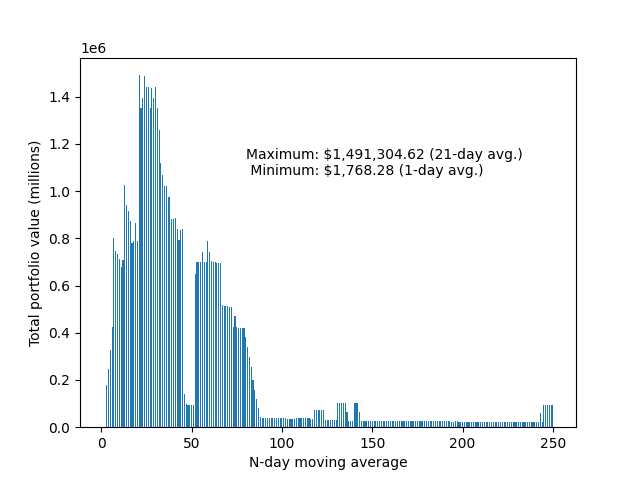
\includegraphics[totalheight=6cm]{mov_avgs.png}
        \centering
        \caption{Plot of 250 different moving averages and their total profits.}
        \label{mov_avgs}
\end{figure*}

\begin{figure*}[h]
    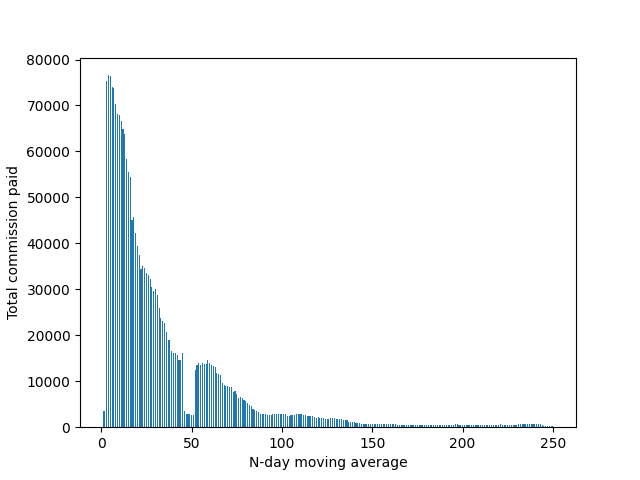
\includegraphics[totalheight=6cm]{commissions.png}
    \centering
    \caption{Plot of 250 different moving averages and their effect on total commission paid.}
    \label{commissions}
\end{figure*}

In Fig.\ (\ref{mov_avgs}), it is apparent that the most successful moving average window is 21 days wide. There is some interesting behavior around the 50-day window mark where profits drop drastically. Further, max profits for window sizes between 75 to 250 are fairly similar with occasional breakouts at the 120, 135, 140, and 245-day marks.
Fig.\ (\ref{commissions}) shows that total commission paid declines consistently as the moving average window size increases. This is expected as smaller windows would result in more volatile averages, which would lead to more trades placed. Again, there is a significant drop around the 50-day window mark that may be of interest to investigate.

\section*{Conclusion}
The best moving average window size is 21 days. There is some strange behavior around the 50-day moving average window, seeing as there is a significant drop in both total profit and commission paid.

\section*{References}
https://pandas.pydata.org/docs/reference/api/pandas.DataFrame.ewm.html
\\\\
https://www.steema.com/docs/financialFunctionsRef/expMovingAverageFunction.htm

\end{document}